\subsection{GWAS Catalog: germline association signal at antigen loci}
\label{sec:gwas}
Somatic and clinical axes so far show a studied-but-undrugged panel; the
germline axis asks whether gated antigen loci also carry population-level
trait or cancer signal. We parsed the full GWAS Catalog ontology-annotated
association file (@NROWS@ associations, latest release; bulk file), assigning
each association to study genes via the mapped-gene column (multi-gene LD
blocks assign to every mapped gene, a caveat kept throughout) and calling
significance at $p\le5\times10^{-8}$.

\paragraph{Calibration gate.} Pre-registered gates PASSED: (G1) PSCA carries
at least one significant cancer-trait association (observed @GATEONE@, the
documented gastric/bladder carcinoma locus); (G2) catalog depth @NROWS@ rows
parsed; (G3) the EGFR sentinel carries at least one significant
cancer-trait association (observed @GATETHREE@).

\paragraph{Any-trait and cancer-trait carriage.} Genes with at least one
significant association: @H1G@/@H1GN@ gated versus @H1B@/@H1BN@ background
(Fisher odds ratio @H1OR@, $p=@H1P@$). Restricting to cancer traits:
@H2G@/@H2GN@ versus @H2B@/@H2BN@ (odds ratio @H2OR@, $p=@H2P@$). Median
significant-association burden is @H3G@ versus @H3B@ (Mann--Whitney
$p=@H3P@$). @VERDICT@

\paragraph{AND-gate antigens.} @ANTIGENBLOCK@

\begin{figure}[t]
\centering
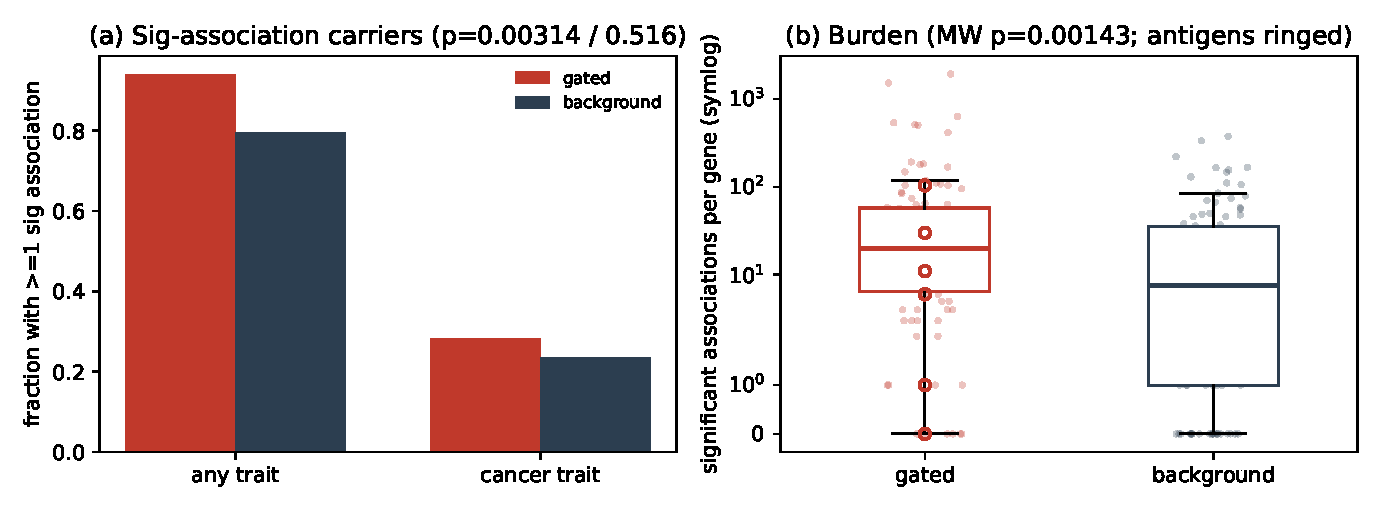
\includegraphics[width=\linewidth]{gwas_fig.pdf}
\caption{GWAS Catalog germline audit. (a) Fraction of genes carrying at
least one genome-wide-significant association, any trait versus cancer
trait. (b) Significant-association burden per gene (symlog axis), with the
seven AND-gate antigens ringed.}
\label{fig:gwas}
\end{figure}
